\chapter{Mapping}
A mapping campaign is planned in the experimental hall, where the n2EDM experiment is going to be located. There are numerous magnetic sources in the vicinity of the site, causing the magnetic environment to be unusually complex. Taking a number of magnetic field maps will provide knowledge necessary to make sure, that the n2EDM compensation system will be able to cope with the environment. A 2.5m high mobile tower with 10 3-axis magnetic field sensors has been constructed. The position and orientation of the tower is measured with cable extension transducers, which makes the mapping process as simple as sweeping an area with the tower. Reproducibility of the maps measured with the device was proven to be better than \SI{0.5}{\micro\tesla}.


\section{The idea}
The precision is not crucial, but the time it takes to measure a map is. The shorter it takes to make a map, the less it is influenced by external conditions. It cannot always be mapped during ,,quiet periods''. We want to have maps of magnetic fields that occur only during busy day-times. For example the crane, or SULTAN or other magnets.

For these reasons it has been decided, that the mapping would consist of a tower. The tower would be moved manually (don't use the future tense here), the position and orientation measured along the magnetic field. Then describe the setup here, briefely. The scalar information is enough to localise sources of magnetic field.

Vector information is useful if the data are to be used for example to calculate dedicated compensation coils for some sources of disturbance.

The setup is shown\ldots The mapper was a tower this and that high, with ten fluxgate magnetometers mounted on it.
The three analogue string potentiometers were mounted on a rigid L-piece. The base element is the string potentiometer. It consists of a wire wound on a spring-loaded spool, the spool attached to a potentiometer. For maximal linearity it is constructed in a way, that the string is wound one in layer only. The string string potentiometers give an analogue signal proportional to the extension of the wire. This information was used to determine the position and orientation of the tower.
\marginpar{Other names for a string potentiometers include: cable-extension transducer, draw-wire sensor and string pot.}
\mnote{The terms like the tower need to be clear by here.}



\section{Principle of a string-potentiometer--based mapper}
For a given signal of a calibrated string potentiometer the points where the free end of the string can be make up a circle. The centre at the location of the body of the sensor, the radius equal to the extension of the wire. In the mapper setup there are two string potentiometers mounted on the fixed L-piece, both extended to a single point on the tower. This points lies on the intersection of the two circles. The problem of determining the location based on the measurement of the distances to a set of fixed points is called \emph{trilateration}.

\marginpar{Other position determination methods include triangulation (measurement of angles between lines connecting a set of fixed points) and multilateration (measurement of the differences of distances between a set of fixed points).}

\begin{figure}
  \centering
  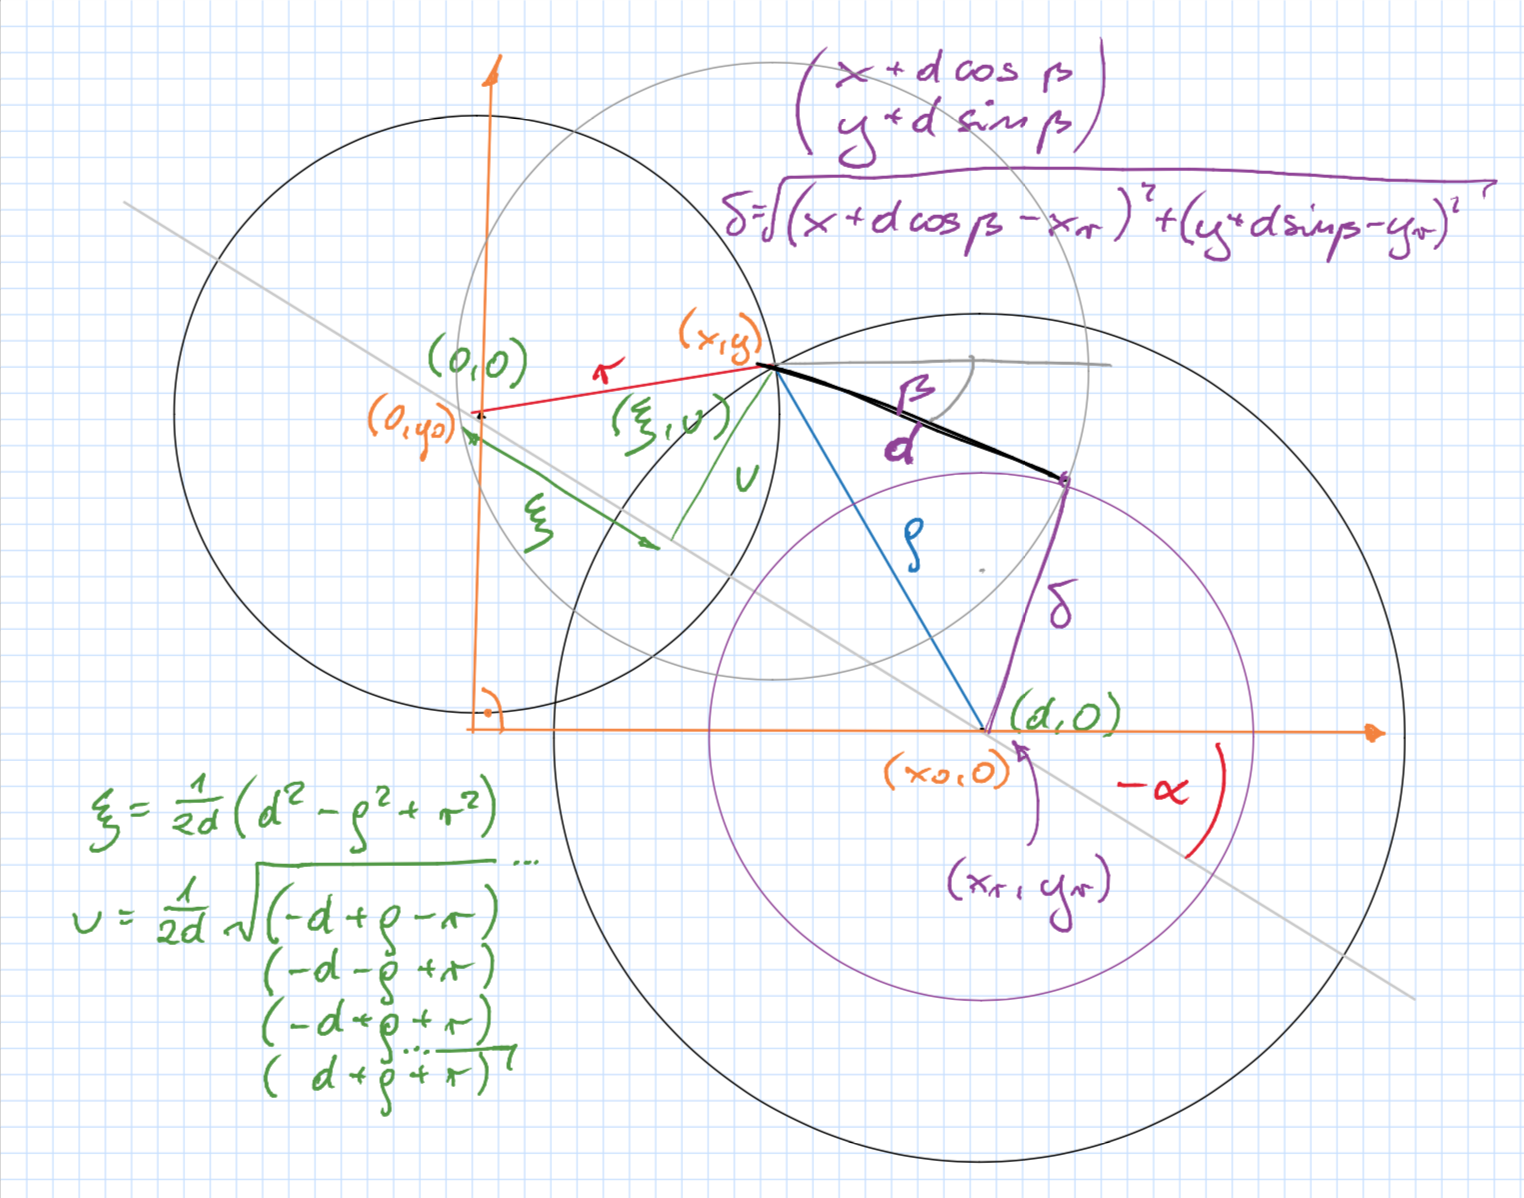
\includegraphics[width=0.9\linewidth]{gfx/mapping/geometry.png}
  \caption{\ldots}
  \label{fig:mapping_geometry}
\end{figure}

The geometry is presented in Fig.\,\ref{fig:mapping_geometry}.The two string potentiometers used to determine the position are located is points $(x, y) = (0, y_0)$ and $(x_0, 0)$ (in the L-piece coordinate system, orange in the figure).
The tower, here point-like, is at $(x,y)$.
The wire extensions are $r$ and $\rho$. For the sake of simplicity, we first give the solution in the coordinate system depicted in green \note{maybe use the A B and C names here already}, where the first string potentiometer is in $(0,0)$ and the second in $(d, 0)$ (with $d = \sqrt{x_0^2 + y_0^2}$). In this coordinate system the tower is in $(\xi, \nu)$.

\begin{align}
  \xi & = \frac{1}{2d} \left( d^2 - \rho^2 + r^2 \right) \\
  \nu & = \frac{1}{2d} \left( (-d + \rho - r) (-d - \rho + r) (-d + \rho + r) (d + \rho + r)  \right)
\end{align}



Let us start with a two-dimensional problem. Span two strings between a magnetic field sensor, each to a fixed position in the room. Based on trilateration. With two strings there are two solutions, but we are always able to detect the correct one.

To get the vector information about the field, also the orientation of the sensors needs to be known. For that an arm can attached to the sensor and a third string spanned to the arm's end.

Now is the time for the nice drawing of the geometry solution.


\section{LPSC campaign}
First the setting. Magnetic characterisation of a new laboratory room, designated for Hg-199 magnetometry research.
A picture of the room (and the mapper, too?).

The setup is shown\ldots The mapper was a tower this and that high, with ten fluxgate magnetometers mounted on it.
The three analogue string potentiometers were mounted on a rigid L-piece (give the positions).
\marginpar{A string potentiometer has a spring-loaded spool attached to a potentiometer. For maximal linearity it is constructed in a way, that the string is wound one layer only.}
\marginpar{Technical details of the setup: fluxgate -- Stefan-Mayer FLC3-70, readout frequency -- xxx, ADC -- aoethu, string potentiometers -- Micro-Eplison xxx}

